\documentclass[1p]{elsarticle_modified}
%\bibliographystyle{elsarticle-num}

%\usepackage[colorlinks]{hyperref}
%\usepackage{abbrmath_seonhwa} %\Abb, \Ascr, \Acal ,\Abf, \Afrak
\usepackage{amsfonts}
\usepackage{amssymb}
\usepackage{amsmath}
\usepackage{amsthm}
\usepackage{scalefnt}
\usepackage{amsbsy}
\usepackage{kotex}
\usepackage{caption}
\usepackage{subfig}
\usepackage{color}
\usepackage{graphicx}
\usepackage{xcolor} %% white, black, red, green, blue, cyan, magenta, yellow
\usepackage{float}
\usepackage{setspace}
\usepackage{hyperref}

\usepackage{tikz}
\usetikzlibrary{arrows}

\usepackage{multirow}
\usepackage{array} % fixed length table
\usepackage{hhline}

%%%%%%%%%%%%%%%%%%%%%
\makeatletter
\renewcommand*\env@matrix[1][\arraystretch]{%
	\edef\arraystretch{#1}%
	\hskip -\arraycolsep
	\let\@ifnextchar\new@ifnextchar
	\array{*\c@MaxMatrixCols c}}
\makeatother %https://tex.stackexchange.com/questions/14071/how-can-i-increase-the-line-spacing-in-a-matrix
%%%%%%%%%%%%%%%

\usepackage[normalem]{ulem}

\newcommand{\msout}[1]{\ifmmode\text{\sout{\ensuremath{#1}}}\else\sout{#1}\fi}
%SOURCE: \msout is \stkout macro in https://tex.stackexchange.com/questions/20609/strikeout-in-math-mode

\newcommand{\cancel}[1]{
	\ifmmode
	{\color{red}\msout{#1}}
	\else
	{\color{red}\sout{#1}}
	\fi
}

\newcommand{\add}[1]{
	{\color{blue}\uwave{#1}}
}

\newcommand{\replace}[2]{
	\ifmmode
	{\color{red}\msout{#1}}{\color{blue}\uwave{#2}}
	\else
	{\color{red}\sout{#1}}{\color{blue}\uwave{#2}}
	\fi
}

\newcommand{\Sol}{\mathcal{S}} %segment
\newcommand{\D}{D} %diagram
\newcommand{\A}{\mathcal{A}} %arc


%%%%%%%%%%%%%%%%%%%%%%%%%%%%%5 test

\def\sl{\operatorname{\textup{SL}}(2,\Cbb)}
\def\psl{\operatorname{\textup{PSL}}(2,\Cbb)}
\def\quan{\mkern 1mu \triangleright \mkern 1mu}

\theoremstyle{definition}
\newtheorem{thm}{Theorem}[section]
\newtheorem{prop}[thm]{Proposition}
\newtheorem{lem}[thm]{Lemma}
\newtheorem{ques}[thm]{Question}
\newtheorem{cor}[thm]{Corollary}
\newtheorem{defn}[thm]{Definition}
\newtheorem{exam}[thm]{Example}
\newtheorem{rmk}[thm]{Remark}
\newtheorem{alg}[thm]{Algorithm}

\newcommand{\I}{\sqrt{-1}}
\begin{document}

%\begin{frontmatter}
%
%\title{Boundary parabolic representations of knots up to 8 crossings}
%
%%% Group authors per affiliation:
%\author{Yunhi Cho} 
%\address{Department of Mathematics, University of Seoul, Seoul, Korea}
%\ead{yhcho@uos.ac.kr}
%
%
%\author{Seonhwa Kim} %\fnref{s_kim}}
%\address{Center for Geometry and Physics, Institute for Basic Science, Pohang, 37673, Korea}
%\ead{ryeona17@ibs.re.kr}
%
%\author{Hyuk Kim}
%\address{Department of Mathematical Sciences, Seoul National University, Seoul 08826, Korea}
%\ead{hyukkim@snu.ac.kr}
%
%\author{Seokbeom Yoon}
%\address{Department of Mathematical Sciences, Seoul National University, Seoul, 08826,  Korea}
%\ead{sbyoon15@snu.ac.kr}
%
%\begin{abstract}
%We find all boundary parabolic representation of knots up to 8 crossings.
%
%\end{abstract}
%\begin{keyword}
%    \MSC[2010] 57M25 
%\end{keyword}
%
%\end{frontmatter}

%\linenumbers
%\tableofcontents
%
\newcommand\colored[1]{\textcolor{white}{\rule[-0.35ex]{0.8em}{1.4ex}}\kern-0.8em\color{red} #1}%
%\newcommand\colored[1]{\textcolor{white}{ #1}\kern-2.17ex	\textcolor{white}{ #1}\kern-1.81ex	\textcolor{white}{ #1}\kern-2.15ex\color{red}#1	}

{\Large $\underline{12n_{0776}~(K12n_{0776})}$}

\setlength{\tabcolsep}{10pt}
\renewcommand{\arraystretch}{1.6}
\vspace{1cm}\begin{tabular}{m{100pt}>{\centering\arraybackslash}m{274pt}}
\multirow{5}{120pt}{
	\centering
	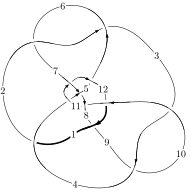
\includegraphics[width=112pt]{../../../GIT/diagram.site/Diagrams/png/2865_12n_0776.png}\\
\ \ \ A knot diagram\footnotemark}&
\allowdisplaybreaks
\textbf{Linearized knot diagam} \\
\cline{2-2}
 &
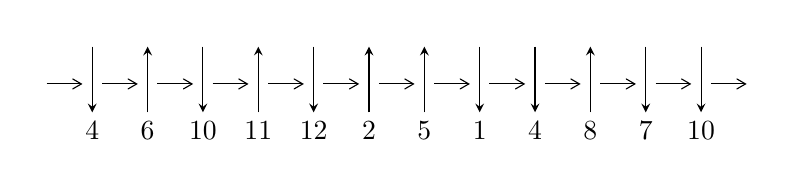
\begin{tikzpicture}[x=20pt, y=17pt]
	% nodes
	\node (C0) at (0, 0) {};
	\node (C1) at (1, 0) {};
	\node (C1U) at (1, +1) {};
	\node (C1D) at (1, -1) {4};

	\node (C2) at (2, 0) {};
	\node (C2U) at (2, +1) {};
	\node (C2D) at (2, -1) {6};

	\node (C3) at (3, 0) {};
	\node (C3U) at (3, +1) {};
	\node (C3D) at (3, -1) {10};

	\node (C4) at (4, 0) {};
	\node (C4U) at (4, +1) {};
	\node (C4D) at (4, -1) {11};

	\node (C5) at (5, 0) {};
	\node (C5U) at (5, +1) {};
	\node (C5D) at (5, -1) {12};

	\node (C6) at (6, 0) {};
	\node (C6U) at (6, +1) {};
	\node (C6D) at (6, -1) {2};

	\node (C7) at (7, 0) {};
	\node (C7U) at (7, +1) {};
	\node (C7D) at (7, -1) {5};

	\node (C8) at (8, 0) {};
	\node (C8U) at (8, +1) {};
	\node (C8D) at (8, -1) {1};

	\node (C9) at (9, 0) {};
	\node (C9U) at (9, +1) {};
	\node (C9D) at (9, -1) {4};

	\node (C10) at (10, 0) {};
	\node (C10U) at (10, +1) {};
	\node (C10D) at (10, -1) {8};

	\node (C11) at (11, 0) {};
	\node (C11U) at (11, +1) {};
	\node (C11D) at (11, -1) {7};

	\node (C12) at (12, 0) {};
	\node (C12U) at (12, +1) {};
	\node (C12D) at (12, -1) {10};
	\node (C13) at (13, 0) {};

	% arrows
	\draw[->,>={angle 60}]
	(C0) edge (C1) (C1) edge (C2) (C2) edge (C3) (C3) edge (C4) (C4) edge (C5) (C5) edge (C6) (C6) edge (C7) (C7) edge (C8) (C8) edge (C9) (C9) edge (C10) (C10) edge (C11) (C11) edge (C12) (C12) edge (C13) ;	\draw[->,>=stealth]
	(C1U) edge (C1D) (C2D) edge (C2U) (C3U) edge (C3D) (C4D) edge (C4U) (C5U) edge (C5D) (C6D) edge (C6U) (C7D) edge (C7U) (C8U) edge (C8D) (C9U) edge (C9D) (C10D) edge (C10U) (C11U) edge (C11D) (C12U) edge (C12D) ;
	\end{tikzpicture} \\
\hhline{~~} \\& 
\textbf{Solving Sequence} \\ \cline{2-2} 
 &
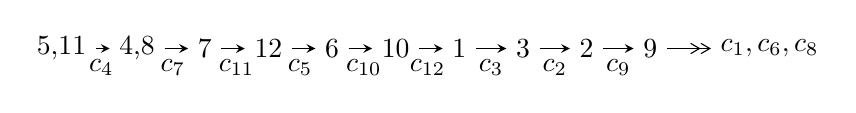
\begin{tikzpicture}[x=23pt, y=7pt]
	% node
	\node (A0) at (-1/8, 0) {5,11};
	\node (A1) at (17/16, 0) {4,8};
	\node (A2) at (17/8, 0) {7};
	\node (A3) at (25/8, 0) {12};
	\node (A4) at (33/8, 0) {6};
	\node (A5) at (41/8, 0) {10};
	\node (A6) at (49/8, 0) {1};
	\node (A7) at (57/8, 0) {3};
	\node (A8) at (65/8, 0) {2};
	\node (A9) at (73/8, 0) {9};
	\node (C1) at (1/2, -1) {$c_{4}$};
	\node (C2) at (13/8, -1) {$c_{7}$};
	\node (C3) at (21/8, -1) {$c_{11}$};
	\node (C4) at (29/8, -1) {$c_{5}$};
	\node (C5) at (37/8, -1) {$c_{10}$};
	\node (C6) at (45/8, -1) {$c_{12}$};
	\node (C7) at (53/8, -1) {$c_{3}$};
	\node (C8) at (61/8, -1) {$c_{2}$};
	\node (C9) at (69/8, -1) {$c_{9}$};
	\node (A10) at (11, 0) {$c_{1},c_{6},c_{8}$};

	% edge
	\draw[->,>=stealth]	
	(A0) edge (A1) (A1) edge (A2) (A2) edge (A3) (A3) edge (A4) (A4) edge (A5) (A5) edge (A6) (A6) edge (A7) (A7) edge (A8) (A8) edge (A9) ;
	\draw[->>,>={angle 60}]	
	(A9) edge (A10);
\end{tikzpicture} \\ 

\end{tabular} \\

\footnotetext{
The image of knot diagram is generated by the software ``\textbf{Draw programme}" developed by Andrew Bartholomew(\url{http://www.layer8.co.uk/maths/draw/index.htm\#Running-draw}), where we modified some parts for our purpose(\url{https://github.com/CATsTAILs/LinksPainter}).
}\phantom \\ \newline 
\centering \textbf{Ideals for irreducible components\footnotemark of $X_{\text{par}}$} 
 
\begin{align*}
I^u_{1}&=\langle 
1.30447\times10^{408} u^{82}+1.37413\times10^{409} u^{81}+\cdots+8.60439\times10^{408} b-2.49025\times10^{408},\\
\phantom{I^u_{1}}&\phantom{= \langle  }-1.05688\times10^{410} u^{82}-1.12073\times10^{411} u^{81}+\cdots+1.29066\times10^{410} a+2.26537\times10^{410},\\
\phantom{I^u_{1}}&\phantom{= \langle  }u^{83}+11 u^{82}+\cdots-13 u-3\rangle \\
I^u_{2}&=\langle 
1.25634\times10^{54} u^{29}+1.27322\times10^{55} u^{28}+\cdots+2.61825\times10^{54} b+1.66292\times10^{54},\\
\phantom{I^u_{2}}&\phantom{= \langle  }2.32992\times10^{54} u^{29}+2.36472\times10^{55} u^{28}+\cdots+3.00141\times10^{54} a+8.04364\times10^{54},\;u^{30}+10 u^{29}+\cdots-2 u+1\rangle \\
\\
\end{align*}
\raggedright * 2 irreducible components of $\dim_{\mathbb{C}}=0$, with total 113 representations.\\
\footnotetext{All coefficients of polynomials are rational numbers. But the coefficients are sometimes approximated in decimal forms when there is not enough margin.}
\newpage
\renewcommand{\arraystretch}{1}
\centering \section*{I. $I^u_{1}= \langle 1.30\times10^{408} u^{82}+1.37\times10^{409} u^{81}+\cdots+8.60\times10^{408} b-2.49\times10^{408},\;-1.06\times10^{410} u^{82}-1.12\times10^{411} u^{81}+\cdots+1.29\times10^{410} a+2.27\times10^{410},\;u^{83}+11 u^{82}+\cdots-13 u-3 \rangle$}
\flushleft \textbf{(i) Arc colorings}\\
\begin{tabular}{m{7pt} m{180pt} m{7pt} m{180pt} }
\flushright $a_{5}=$&$\begin{pmatrix}1\\0\end{pmatrix}$ \\
\flushright $a_{11}=$&$\begin{pmatrix}0\\u\end{pmatrix}$ \\
\flushright $a_{4}=$&$\begin{pmatrix}1\\u^2\end{pmatrix}$ \\
\flushright $a_{8}=$&$\begin{pmatrix}0.818869 u^{82}+8.68343 u^{81}+\cdots+28.1044 u-1.75521\\-0.151605 u^{82}-1.59701 u^{81}+\cdots+2.31640 u+0.289416\end{pmatrix}$ \\
\flushright $a_{7}=$&$\begin{pmatrix}0.970473 u^{82}+10.2804 u^{81}+\cdots+25.7880 u-2.04462\\-0.151605 u^{82}-1.59701 u^{81}+\cdots+2.31640 u+0.289416\end{pmatrix}$ \\
\flushright $a_{12}=$&$\begin{pmatrix}-0.751807 u^{82}-7.77308 u^{81}+\cdots+119.279 u+25.5349\\-0.0208145 u^{82}-0.206503 u^{81}+\cdots-1.29505 u-1.10729\end{pmatrix}$ \\
\flushright $a_{6}=$&$\begin{pmatrix}0.0172443 u^{82}-0.0375127 u^{81}+\cdots-126.673 u-18.4506\\-0.0490051 u^{82}-0.539643 u^{81}+\cdots+3.70028 u+1.39331\end{pmatrix}$ \\
\flushright $a_{10}=$&$\begin{pmatrix}-0.731904 u^{82}-7.54031 u^{81}+\cdots+113.239 u+23.1711\\0.0407173 u^{82}+0.439275 u^{81}+\cdots-2.74464 u-1.25654\end{pmatrix}$ \\
\flushright $a_{1}=$&$\begin{pmatrix}-1.19729 u^{82}-12.6448 u^{81}+\cdots+1.47287 u+12.3678\\-0.0211191 u^{82}-0.198672 u^{81}+\cdots+2.33013 u-0.629956\end{pmatrix}$ \\
\flushright $a_{3}=$&$\begin{pmatrix}-2.19019 u^{82}-23.7541 u^{81}+\cdots+139.252 u+18.1407\\0.108002 u^{82}+1.16613 u^{81}+\cdots-5.31878 u-1.13687\end{pmatrix}$ \\
\flushright $a_{2}=$&$\begin{pmatrix}-1.26772 u^{82}-13.4375 u^{81}+\cdots+2.38069 u+14.5739\\-0.00603930 u^{82}-0.0390650 u^{81}+\cdots+1.88614 u-0.683654\end{pmatrix}$ \\
\flushright $a_{9}=$&$\begin{pmatrix}-0.532288 u^{82}-5.37650 u^{81}+\cdots+106.052 u+20.3826\\0.0409161 u^{82}+0.446102 u^{81}+\cdots-2.56150 u-1.35247\end{pmatrix}$\\&\end{tabular}
\flushleft \textbf{(ii) Obstruction class $= -1$}\\~\\
\flushleft \textbf{(iii) Cusp Shapes $= 1.65712 u^{82}+17.5491 u^{81}+\cdots-136.696 u-33.9475$}\\~\\
\newpage\renewcommand{\arraystretch}{1}
\flushleft \textbf{(iv) u-Polynomials at the component}\newline \\
\begin{tabular}{m{50pt}|m{274pt}}
Crossings & \hspace{64pt}u-Polynomials at each crossing \\
\hline $$\begin{aligned}c_{1}\end{aligned}$$&$\begin{aligned}
&u^{83}+u^{82}+\cdots-53405 u+3225
\end{aligned}$\\
\hline $$\begin{aligned}c_{2},c_{6}\end{aligned}$$&$\begin{aligned}
&u^{83}+2 u^{82}+\cdots+217 u-67
\end{aligned}$\\
\hline $$\begin{aligned}c_{3},c_{9}\end{aligned}$$&$\begin{aligned}
&u^{83}+10 u^{82}+\cdots+34163451 u-6221089
\end{aligned}$\\
\hline $$\begin{aligned}c_{4}\end{aligned}$$&$\begin{aligned}
&u^{83}+11 u^{82}+\cdots-13 u-3
\end{aligned}$\\
\hline $$\begin{aligned}c_{5}\end{aligned}$$&$\begin{aligned}
&u^{83}-15 u^{81}+\cdots-486505 u+43627
\end{aligned}$\\
\hline $$\begin{aligned}c_{7}\end{aligned}$$&$\begin{aligned}
&u^{83}+5 u^{82}+\cdots-6 u-1
\end{aligned}$\\
\hline $$\begin{aligned}c_{8}\end{aligned}$$&$\begin{aligned}
&u^{83}-51 u^{81}+\cdots+17717265 u-4973081
\end{aligned}$\\
\hline $$\begin{aligned}c_{10}\end{aligned}$$&$\begin{aligned}
&u^{83}+11 u^{82}+\cdots+1754 u+107
\end{aligned}$\\
\hline $$\begin{aligned}c_{11}\end{aligned}$$&$\begin{aligned}
&u^{83}+7 u^{82}+\cdots-3609 u+331
\end{aligned}$\\
\hline $$\begin{aligned}c_{12}\end{aligned}$$&$\begin{aligned}
&u^{83}-11 u^{82}+\cdots+133746194 u+15906677
\end{aligned}$\\
\hline
\end{tabular}\\~\\
\newpage\renewcommand{\arraystretch}{1}
\flushleft \textbf{(v) Riley Polynomials at the component}\newline \\
\begin{tabular}{m{50pt}|m{274pt}}
Crossings & \hspace{64pt}Riley Polynomials at each crossing \\
\hline $$\begin{aligned}c_{1}\end{aligned}$$&$\begin{aligned}
&y^{83}-131 y^{82}+\cdots-220531175 y-10400625
\end{aligned}$\\
\hline $$\begin{aligned}c_{2},c_{6}\end{aligned}$$&$\begin{aligned}
&y^{83}+60 y^{82}+\cdots-303187 y-4489
\end{aligned}$\\
\hline $$\begin{aligned}c_{3},c_{9}\end{aligned}$$&$\begin{aligned}
&y^{83}-126 y^{82}+\cdots-86541304996979 y-38701948345921
\end{aligned}$\\
\hline $$\begin{aligned}c_{4}\end{aligned}$$&$\begin{aligned}
&y^{83}-15 y^{82}+\cdots+7 y-9
\end{aligned}$\\
\hline $$\begin{aligned}c_{5}\end{aligned}$$&$\begin{aligned}
&y^{83}-30 y^{82}+\cdots+62663810995 y-1903315129
\end{aligned}$\\
\hline $$\begin{aligned}c_{7}\end{aligned}$$&$\begin{aligned}
&y^{83}+13 y^{82}+\cdots-96 y-1
\end{aligned}$\\
\hline $$\begin{aligned}c_{8}\end{aligned}$$&$\begin{aligned}
&y^{83}-102 y^{82}+\cdots-98203788924489 y-24731534632561
\end{aligned}$\\
\hline $$\begin{aligned}c_{10}\end{aligned}$$&$\begin{aligned}
&y^{83}+17 y^{82}+\cdots-583740 y-11449
\end{aligned}$\\
\hline $$\begin{aligned}c_{11}\end{aligned}$$&$\begin{aligned}
&y^{83}+5 y^{82}+\cdots+2855899 y-109561
\end{aligned}$\\
\hline $$\begin{aligned}c_{12}\end{aligned}$$&$\begin{aligned}
&y^{83}-303 y^{82}+\cdots-13069623167467982 y-253022373182329
\end{aligned}$\\
\hline
\end{tabular}\\~\\
\newpage\flushleft \textbf{(vi) Complex Volumes and Cusp Shapes}
$$\begin{array}{c|c|c}  
\text{Solutions to }I^u_{1}& \I (\text{vol} + \sqrt{-1}CS) & \text{Cusp shape}\\
 \hline 
\begin{aligned}
u &= \phantom{-}0.709906 + 0.690044 I \\
a &= -0.927762 + 0.065003 I \\
b &= -1.090150 + 0.433533 I\end{aligned}
 & -0.98312 + 1.83332 I & \phantom{-0.000000 } 0 \\ \hline\begin{aligned}
u &= \phantom{-}0.709906 - 0.690044 I \\
a &= -0.927762 - 0.065003 I \\
b &= -1.090150 - 0.433533 I\end{aligned}
 & -0.98312 - 1.83332 I & \phantom{-0.000000 } 0 \\ \hline\begin{aligned}
u &= \phantom{-}0.261828 + 0.930528 I \\
a &= -0.764997 + 0.206710 I \\
b &= -0.298237 + 0.061397 I\end{aligned}
 & -0.40627 + 1.72494 I & \phantom{-0.000000 } 0 \\ \hline\begin{aligned}
u &= \phantom{-}0.261828 - 0.930528 I \\
a &= -0.764997 - 0.206710 I \\
b &= -0.298237 - 0.061397 I\end{aligned}
 & -0.40627 - 1.72494 I & \phantom{-0.000000 } 0 \\ \hline\begin{aligned}
u &= -0.894847 + 0.518321 I \\
a &= \phantom{-}1.59094 - 0.23930 I \\
b &= \phantom{-}1.118840 - 0.816514 I\end{aligned}
 & \phantom{-}3.48501 - 4.70122 I & \phantom{-0.000000 } 0 \\ \hline\begin{aligned}
u &= -0.894847 - 0.518321 I \\
a &= \phantom{-}1.59094 + 0.23930 I \\
b &= \phantom{-}1.118840 + 0.816514 I\end{aligned}
 & \phantom{-}3.48501 + 4.70122 I & \phantom{-0.000000 } 0 \\ \hline\begin{aligned}
u &= -0.362153 + 0.892735 I \\
a &= \phantom{-}1.38780 + 0.53803 I \\
b &= -0.181923 - 0.485373 I\end{aligned}
 & -3.04231 + 1.75204 I & \phantom{-0.000000 } 0 \\ \hline\begin{aligned}
u &= -0.362153 - 0.892735 I \\
a &= \phantom{-}1.38780 - 0.53803 I \\
b &= -0.181923 + 0.485373 I\end{aligned}
 & -3.04231 - 1.75204 I & \phantom{-0.000000 } 0 \\ \hline\begin{aligned}
u &= -0.740237 + 0.744539 I \\
a &= -0.421844 + 0.182382 I \\
b &= -0.823000 + 0.195896 I\end{aligned}
 & -0.28428 + 2.31145 I & \phantom{-0.000000 } 0 \\ \hline\begin{aligned}
u &= -0.740237 - 0.744539 I \\
a &= -0.421844 - 0.182382 I \\
b &= -0.823000 - 0.195896 I\end{aligned}
 & -0.28428 - 2.31145 I & \phantom{-0.000000 } 0\\
 \hline 
 \end{array}$$\newpage$$\begin{array}{c|c|c}  
\text{Solutions to }I^u_{1}& \I (\text{vol} + \sqrt{-1}CS) & \text{Cusp shape}\\
 \hline 
\begin{aligned}
u &= \phantom{-}0.270866 + 1.053850 I \\
a &= \phantom{-}1.49395 - 0.74055 I \\
b &= \phantom{-}0.081067 + 0.787778 I\end{aligned}
 & -13.4588 + 7.1690 I & \phantom{-0.000000 } 0 \\ \hline\begin{aligned}
u &= \phantom{-}0.270866 - 1.053850 I \\
a &= \phantom{-}1.49395 + 0.74055 I \\
b &= \phantom{-}0.081067 - 0.787778 I\end{aligned}
 & -13.4588 - 7.1690 I & \phantom{-0.000000 } 0 \\ \hline\begin{aligned}
u &= -0.758010 + 0.437224 I \\
a &= -1.44879 - 1.65189 I \\
b &= -0.791564 + 0.668716 I\end{aligned}
 & -9.72538 - 8.72357 I & \phantom{-0.000000 } 0 \\ \hline\begin{aligned}
u &= -0.758010 - 0.437224 I \\
a &= -1.44879 + 1.65189 I \\
b &= -0.791564 - 0.668716 I\end{aligned}
 & -9.72538 + 8.72357 I & \phantom{-0.000000 } 0 \\ \hline\begin{aligned}
u &= -0.516399 + 0.659806 I \\
a &= -0.798299 + 0.327613 I \\
b &= -0.75838 + 1.49622 I\end{aligned}
 & -5.06876 - 0.94779 I & \phantom{-0.000000 } 0 \\ \hline\begin{aligned}
u &= -0.516399 - 0.659806 I \\
a &= -0.798299 - 0.327613 I \\
b &= -0.75838 - 1.49622 I\end{aligned}
 & -5.06876 + 0.94779 I & \phantom{-0.000000 } 0 \\ \hline\begin{aligned}
u &= -0.602229 + 0.994072 I \\
a &= -1.45123 - 0.15027 I \\
b &= -0.92859 + 1.10832 I\end{aligned}
 & -14.0609 - 2.5251 I & \phantom{-0.000000 } 0 \\ \hline\begin{aligned}
u &= -0.602229 - 0.994072 I \\
a &= -1.45123 + 0.15027 I \\
b &= -0.92859 - 1.10832 I\end{aligned}
 & -14.0609 + 2.5251 I & \phantom{-0.000000 } 0 \\ \hline\begin{aligned}
u &= \phantom{-}0.803341 + 0.845356 I \\
a &= -0.913620 - 0.197343 I \\
b &= -0.280226 - 0.440104 I\end{aligned}
 & -0.29002 + 2.15185 I & \phantom{-0.000000 } 0 \\ \hline\begin{aligned}
u &= \phantom{-}0.803341 - 0.845356 I \\
a &= -0.913620 + 0.197343 I \\
b &= -0.280226 + 0.440104 I\end{aligned}
 & -0.29002 - 2.15185 I & \phantom{-0.000000 } 0\\
 \hline 
 \end{array}$$\newpage$$\begin{array}{c|c|c}  
\text{Solutions to }I^u_{1}& \I (\text{vol} + \sqrt{-1}CS) & \text{Cusp shape}\\
 \hline 
\begin{aligned}
u &= \phantom{-}0.680380 + 0.437401 I \\
a &= \phantom{-}0.501491 - 0.074945 I \\
b &= \phantom{-}0.824171 + 0.728489 I\end{aligned}
 & \phantom{-}1.37263 + 1.70785 I & \phantom{-0.000000 } 0 \\ \hline\begin{aligned}
u &= \phantom{-}0.680380 - 0.437401 I \\
a &= \phantom{-}0.501491 + 0.074945 I \\
b &= \phantom{-}0.824171 - 0.728489 I\end{aligned}
 & \phantom{-}1.37263 - 1.70785 I & \phantom{-0.000000 } 0 \\ \hline\begin{aligned}
u &= -0.233492 + 0.754653 I \\
a &= -1.000650 + 0.119961 I \\
b &= \phantom{-}0.060779 + 0.557525 I\end{aligned}
 & -1.09485 + 1.14990 I & \phantom{-0.000000 } 0 \\ \hline\begin{aligned}
u &= -0.233492 - 0.754653 I \\
a &= -1.000650 - 0.119961 I \\
b &= \phantom{-}0.060779 - 0.557525 I\end{aligned}
 & -1.09485 - 1.14990 I & \phantom{-0.000000 } 0 \\ \hline\begin{aligned}
u &= -0.577250 + 0.501896 I \\
a &= -1.42505 + 0.21771 I \\
b &= -1.60916 - 0.88816 I\end{aligned}
 & -10.73260 - 8.88187 I & \phantom{-0.000000 -}0. + 8.54488 I \\ \hline\begin{aligned}
u &= -0.577250 - 0.501896 I \\
a &= -1.42505 - 0.21771 I \\
b &= -1.60916 + 0.88816 I\end{aligned}
 & -10.73260 + 8.88187 I & \phantom{-0.000000 } 0. - 8.54488 I \\ \hline\begin{aligned}
u &= \phantom{-}0.777187 + 1.003380 I \\
a &= -1.057860 - 0.100809 I \\
b &= -1.08433 - 1.22178 I\end{aligned}
 & -4.76888 + 8.66641 I & \phantom{-0.000000 } 0 \\ \hline\begin{aligned}
u &= \phantom{-}0.777187 - 1.003380 I \\
a &= -1.057860 + 0.100809 I \\
b &= -1.08433 + 1.22178 I\end{aligned}
 & -4.76888 - 8.66641 I & \phantom{-0.000000 } 0 \\ \hline\begin{aligned}
u &= \phantom{-}0.064315 + 1.270220 I \\
a &= -0.687278 - 0.229993 I \\
b &= -1.19350 - 1.01922 I\end{aligned}
 & -13.2417 + 5.2799 I & \phantom{-0.000000 } 0 \\ \hline\begin{aligned}
u &= \phantom{-}0.064315 - 1.270220 I \\
a &= -0.687278 + 0.229993 I \\
b &= -1.19350 + 1.01922 I\end{aligned}
 & -13.2417 - 5.2799 I & \phantom{-0.000000 } 0\\
 \hline 
 \end{array}$$\newpage$$\begin{array}{c|c|c}  
\text{Solutions to }I^u_{1}& \I (\text{vol} + \sqrt{-1}CS) & \text{Cusp shape}\\
 \hline 
\begin{aligned}
u &= -0.680427 + 0.042583 I \\
a &= \phantom{-}1.38569 + 0.95422 I \\
b &= \phantom{-}1.098090 - 0.661662 I\end{aligned}
 & \phantom{-}3.67022 - 0.24922 I & \phantom{-}11.72806 - 2.38470 I \\ \hline\begin{aligned}
u &= -0.680427 - 0.042583 I \\
a &= \phantom{-}1.38569 - 0.95422 I \\
b &= \phantom{-}1.098090 + 0.661662 I\end{aligned}
 & \phantom{-}3.67022 + 0.24922 I & \phantom{-}11.72806 + 2.38470 I \\ \hline\begin{aligned}
u &= \phantom{-}0.948869 + 0.927196 I \\
a &= \phantom{-}0.689941 + 0.118533 I \\
b &= \phantom{-}0.820966 + 1.116060 I\end{aligned}
 & \phantom{-}0.03269 + 4.50461 I & \phantom{-0.000000 } 0 \\ \hline\begin{aligned}
u &= \phantom{-}0.948869 - 0.927196 I \\
a &= \phantom{-}0.689941 - 0.118533 I \\
b &= \phantom{-}0.820966 - 1.116060 I\end{aligned}
 & \phantom{-}0.03269 - 4.50461 I & \phantom{-0.000000 } 0 \\ \hline\begin{aligned}
u &= -0.574607 + 0.326079 I \\
a &= \phantom{-}1.81871 - 0.33275 I \\
b &= \phantom{-}1.25086 - 1.16436 I\end{aligned}
 & \phantom{-}2.26604 - 3.57767 I & -8.97068 + 8.43068 I \\ \hline\begin{aligned}
u &= -0.574607 - 0.326079 I \\
a &= \phantom{-}1.81871 + 0.33275 I \\
b &= \phantom{-}1.25086 + 1.16436 I\end{aligned}
 & \phantom{-}2.26604 + 3.57767 I & -8.97068 - 8.43068 I \\ \hline\begin{aligned}
u &= \phantom{-}0.927408 + 0.976224 I \\
a &= -0.319524 - 0.705776 I \\
b &= \phantom{-}0.160830 - 0.946290 I\end{aligned}
 & -8.05970 - 2.70904 I & \phantom{-0.000000 } 0 \\ \hline\begin{aligned}
u &= \phantom{-}0.927408 - 0.976224 I \\
a &= -0.319524 + 0.705776 I \\
b &= \phantom{-}0.160830 + 0.946290 I\end{aligned}
 & -8.05970 + 2.70904 I & \phantom{-0.000000 } 0 \\ \hline\begin{aligned}
u &= \phantom{-}0.373196 + 0.449963 I \\
a &= \phantom{-}1.72772 + 1.13860 I \\
b &= \phantom{-}0.447128 - 1.280330 I\end{aligned}
 & -10.82210 + 1.04215 I & -8.95659 - 0.64479 I \\ \hline\begin{aligned}
u &= \phantom{-}0.373196 - 0.449963 I \\
a &= \phantom{-}1.72772 - 1.13860 I \\
b &= \phantom{-}0.447128 + 1.280330 I\end{aligned}
 & -10.82210 - 1.04215 I & -8.95659 + 0.64479 I\\
 \hline 
 \end{array}$$\newpage$$\begin{array}{c|c|c}  
\text{Solutions to }I^u_{1}& \I (\text{vol} + \sqrt{-1}CS) & \text{Cusp shape}\\
 \hline 
\begin{aligned}
u &= \phantom{-}1.02114 + 1.01195 I \\
a &= \phantom{-}1.165700 + 0.230472 I \\
b &= \phantom{-}0.99942 + 1.24394 I\end{aligned}
 & -7.91150 + 10.06580 I & \phantom{-0.000000 } 0 \\ \hline\begin{aligned}
u &= \phantom{-}1.02114 - 1.01195 I \\
a &= \phantom{-}1.165700 - 0.230472 I \\
b &= \phantom{-}0.99942 - 1.24394 I\end{aligned}
 & -7.91150 - 10.06580 I & \phantom{-0.000000 } 0 \\ \hline\begin{aligned}
u &= -0.165432 + 0.479272 I \\
a &= \phantom{-}1.74495 - 1.61770 I \\
b &= -0.331671 + 0.790672 I\end{aligned}
 & -2.95336 - 5.09545 I & -6.33229 + 9.13394 I \\ \hline\begin{aligned}
u &= -0.165432 - 0.479272 I \\
a &= \phantom{-}1.74495 + 1.61770 I \\
b &= -0.331671 - 0.790672 I\end{aligned}
 & -2.95336 + 5.09545 I & -6.33229 - 9.13394 I \\ \hline\begin{aligned}
u &= \phantom{-}0.504156\phantom{ +0.000000I} \\
a &= \phantom{-}5.40046\phantom{ +0.000000I} \\
b &= \phantom{-}0.696000\phantom{ +0.000000I}\end{aligned}
 & -4.71616\phantom{ +0.000000I} & \phantom{-}10.6220\phantom{ +0.000000I} \\ \hline\begin{aligned}
u &= \phantom{-}0.10860 + 1.51156 I \\
a &= \phantom{-}0.484440 + 0.127681 I \\
b &= \phantom{-}1.002370 + 0.085521 I\end{aligned}
 & \phantom{-}0.309078 + 0.377421 I & \phantom{-0.000000 } 0 \\ \hline\begin{aligned}
u &= \phantom{-}0.10860 - 1.51156 I \\
a &= \phantom{-}0.484440 - 0.127681 I \\
b &= \phantom{-}1.002370 - 0.085521 I\end{aligned}
 & \phantom{-}0.309078 - 0.377421 I & \phantom{-0.000000 } 0 \\ \hline\begin{aligned}
u &= -1.31990 + 0.75395 I \\
a &= \phantom{-}0.861735 - 0.367052 I \\
b &= \phantom{-}0.90290 - 1.18899 I\end{aligned}
 & \phantom{-}2.06751 - 7.02731 I & \phantom{-0.000000 } 0 \\ \hline\begin{aligned}
u &= -1.31990 - 0.75395 I \\
a &= \phantom{-}0.861735 + 0.367052 I \\
b &= \phantom{-}0.90290 + 1.18899 I\end{aligned}
 & \phantom{-}2.06751 + 7.02731 I & \phantom{-0.000000 } 0 \\ \hline\begin{aligned}
u &= -1.03049 + 1.12737 I \\
a &= -0.670023 + 0.083173 I \\
b &= -0.799015 + 1.128390 I\end{aligned}
 & -2.24741 - 9.70482 I & \phantom{-0.000000 } 0\\
 \hline 
 \end{array}$$\newpage$$\begin{array}{c|c|c}  
\text{Solutions to }I^u_{1}& \I (\text{vol} + \sqrt{-1}CS) & \text{Cusp shape}\\
 \hline 
\begin{aligned}
u &= -1.03049 - 1.12737 I \\
a &= -0.670023 - 0.083173 I \\
b &= -0.799015 - 1.128390 I\end{aligned}
 & -2.24741 + 9.70482 I & \phantom{-0.000000 } 0 \\ \hline\begin{aligned}
u &= -1.02629 + 1.15598 I \\
a &= -0.816028 + 0.211399 I \\
b &= -0.677550 + 0.597699 I\end{aligned}
 & -5.06471 - 5.76701 I & \phantom{-0.000000 } 0 \\ \hline\begin{aligned}
u &= -1.02629 - 1.15598 I \\
a &= -0.816028 - 0.211399 I \\
b &= -0.677550 - 0.597699 I\end{aligned}
 & -5.06471 + 5.76701 I & \phantom{-0.000000 } 0 \\ \hline\begin{aligned}
u &= \phantom{-}1.36893 + 0.74159 I \\
a &= \phantom{-}0.399726 - 0.420329 I \\
b &= \phantom{-}0.578099 + 0.577904 I\end{aligned}
 & -5.53407 + 1.96330 I & \phantom{-0.000000 } 0 \\ \hline\begin{aligned}
u &= \phantom{-}1.36893 - 0.74159 I \\
a &= \phantom{-}0.399726 + 0.420329 I \\
b &= \phantom{-}0.578099 - 0.577904 I\end{aligned}
 & -5.53407 - 1.96330 I & \phantom{-0.000000 } 0 \\ \hline\begin{aligned}
u &= \phantom{-}0.043734 + 0.437894 I \\
a &= \phantom{-}1.37494 - 0.86927 I \\
b &= \phantom{-}1.80634 - 1.67583 I\end{aligned}
 & -6.61873 + 0.72943 I & -27.0371 - 3.0253 I \\ \hline\begin{aligned}
u &= \phantom{-}0.043734 - 0.437894 I \\
a &= \phantom{-}1.37494 + 0.86927 I \\
b &= \phantom{-}1.80634 + 1.67583 I\end{aligned}
 & -6.61873 - 0.72943 I & -27.0371 + 3.0253 I \\ \hline\begin{aligned}
u &= -1.48630 + 0.49749 I \\
a &= -0.184899 - 0.725570 I \\
b &= -0.514333 - 1.079950 I\end{aligned}
 & -11.23120 - 3.55868 I & \phantom{-0.000000 } 0 \\ \hline\begin{aligned}
u &= -1.48630 - 0.49749 I \\
a &= -0.184899 + 0.725570 I \\
b &= -0.514333 + 1.079950 I\end{aligned}
 & -11.23120 + 3.55868 I & \phantom{-0.000000 } 0 \\ \hline\begin{aligned}
u &= \phantom{-}1.17287 + 1.06491 I \\
a &= -0.948428 - 0.052602 I \\
b &= -0.770986 - 1.135900 I\end{aligned}
 & -2.90730 + 8.25650 I & \phantom{-0.000000 } 0\\
 \hline 
 \end{array}$$\newpage$$\begin{array}{c|c|c}  
\text{Solutions to }I^u_{1}& \I (\text{vol} + \sqrt{-1}CS) & \text{Cusp shape}\\
 \hline 
\begin{aligned}
u &= \phantom{-}1.17287 - 1.06491 I \\
a &= -0.948428 + 0.052602 I \\
b &= -0.770986 + 1.135900 I\end{aligned}
 & -2.90730 - 8.25650 I & \phantom{-0.000000 } 0 \\ \hline\begin{aligned}
u &= \phantom{-}1.60080 + 0.00259 I \\
a &= -0.308479 + 0.601802 I \\
b &= -0.512848 + 0.469068 I\end{aligned}
 & -2.12534 - 2.73496 I & \phantom{-0.000000 } 0 \\ \hline\begin{aligned}
u &= \phantom{-}1.60080 - 0.00259 I \\
a &= -0.308479 - 0.601802 I \\
b &= -0.512848 - 0.469068 I\end{aligned}
 & -2.12534 + 2.73496 I & \phantom{-0.000000 } 0 \\ \hline\begin{aligned}
u &= -0.275291 + 0.221049 I \\
a &= -0.64665 + 1.27043 I \\
b &= -1.054180 - 0.813914 I\end{aligned}
 & -0.89305 - 2.92243 I & -9.70267 + 2.02248 I \\ \hline\begin{aligned}
u &= -0.275291 - 0.221049 I \\
a &= -0.64665 - 1.27043 I \\
b &= -1.054180 + 0.813914 I\end{aligned}
 & -0.89305 + 2.92243 I & -9.70267 - 2.02248 I \\ \hline\begin{aligned}
u &= -0.318817 + 0.131695 I \\
a &= -3.73118 - 2.56355 I \\
b &= \phantom{-}0.0551272 + 0.0990377 I\end{aligned}
 & -2.40668 - 0.00982 I & -16.7035 - 7.8985 I \\ \hline\begin{aligned}
u &= -0.318817 - 0.131695 I \\
a &= -3.73118 + 2.56355 I \\
b &= \phantom{-}0.0551272 - 0.0990377 I\end{aligned}
 & -2.40668 + 0.00982 I & -16.7035 + 7.8985 I \\ \hline\begin{aligned}
u &= \phantom{-}0.252941 + 0.222750 I \\
a &= -1.61194 - 2.97824 I \\
b &= -0.203176 - 1.245190 I\end{aligned}
 & -7.63133 - 1.98716 I & -11.03642 + 4.01004 I \\ \hline\begin{aligned}
u &= \phantom{-}0.252941 - 0.222750 I \\
a &= -1.61194 + 2.97824 I \\
b &= -0.203176 + 1.245190 I\end{aligned}
 & -7.63133 + 1.98716 I & -11.03642 - 4.01004 I \\ \hline\begin{aligned}
u &= -1.20089 + 1.18117 I \\
a &= -0.951427 + 0.190149 I \\
b &= -0.97977 + 1.25279 I\end{aligned}
 & -12.3596 - 17.5347 I & \phantom{-0.000000 } 0\\
 \hline 
 \end{array}$$\newpage$$\begin{array}{c|c|c}  
\text{Solutions to }I^u_{1}& \I (\text{vol} + \sqrt{-1}CS) & \text{Cusp shape}\\
 \hline 
\begin{aligned}
u &= -1.20089 - 1.18117 I \\
a &= -0.951427 - 0.190149 I \\
b &= -0.97977 - 1.25279 I\end{aligned}
 & -12.3596 + 17.5347 I & \phantom{-0.000000 } 0 \\ \hline\begin{aligned}
u &= \phantom{-}0.40829 + 1.64602 I \\
a &= \phantom{-}0.252064 - 0.072091 I \\
b &= -0.082371 + 0.853035 I\end{aligned}
 & -4.39323 + 0.59906 I & \phantom{-0.000000 } 0 \\ \hline\begin{aligned}
u &= \phantom{-}0.40829 - 1.64602 I \\
a &= \phantom{-}0.252064 + 0.072091 I \\
b &= -0.082371 - 0.853035 I\end{aligned}
 & -4.39323 - 0.59906 I & \phantom{-0.000000 } 0 \\ \hline\begin{aligned}
u &= \phantom{-}0.133270 + 0.145455 I \\
a &= \phantom{-}1.89268 + 13.71840 I \\
b &= -0.154111 - 0.408727 I\end{aligned}
 & -2.72551 - 0.66144 I & -24.1115 - 31.0038 I \\ \hline\begin{aligned}
u &= \phantom{-}0.133270 - 0.145455 I \\
a &= \phantom{-}1.89268 - 13.71840 I \\
b &= -0.154111 + 0.408727 I\end{aligned}
 & -2.72551 + 0.66144 I & -24.1115 + 31.0038 I \\ \hline\begin{aligned}
u &= -1.57118 + 0.94094 I \\
a &= \phantom{-}0.451176 - 0.364575 I \\
b &= \phantom{-}0.294701 - 0.688444 I\end{aligned}
 & -2.17859 - 4.62625 I & \phantom{-0.000000 } 0 \\ \hline\begin{aligned}
u &= -1.57118 - 0.94094 I \\
a &= \phantom{-}0.451176 + 0.364575 I \\
b &= \phantom{-}0.294701 + 0.688444 I\end{aligned}
 & -2.17859 + 4.62625 I & \phantom{-0.000000 } 0 \\ \hline\begin{aligned}
u &= \phantom{-}1.16083 + 1.45232 I \\
a &= \phantom{-}0.665646 + 0.142507 I \\
b &= \phantom{-}1.033180 + 0.595503 I\end{aligned}
 & -8.06942 + 7.08098 I & \phantom{-0.000000 } 0 \\ \hline\begin{aligned}
u &= \phantom{-}1.16083 - 1.45232 I \\
a &= \phantom{-}0.665646 - 0.142507 I \\
b &= \phantom{-}1.033180 - 0.595503 I\end{aligned}
 & -8.06942 - 7.08098 I & \phantom{-0.000000 } 0 \\ \hline\begin{aligned}
u &= -1.20226 + 1.73624 I \\
a &= \phantom{-}0.213848 - 0.358282 I \\
b &= -0.247627 - 0.670148 I\end{aligned}
 & -12.8693 + 7.8727 I & \phantom{-0.000000 } 0\\
 \hline 
 \end{array}$$\newpage$$\begin{array}{c|c|c}  
\text{Solutions to }I^u_{1}& \I (\text{vol} + \sqrt{-1}CS) & \text{Cusp shape}\\
 \hline 
\begin{aligned}
u &= -1.20226 - 1.73624 I \\
a &= \phantom{-}0.213848 + 0.358282 I \\
b &= -0.247627 + 0.670148 I\end{aligned}
 & -12.8693 - 7.8727 I & \phantom{-0.000000 } 0 \\ \hline\begin{aligned}
u &= -3.30429 + 0.71948 I \\
a &= -0.0507409 + 0.0686539 I \\
b &= -0.016178 + 1.084750 I\end{aligned}
 & -4.67503 + 0.08868 I & \phantom{-0.000000 } 0 \\ \hline\begin{aligned}
u &= -3.30429 - 0.71948 I \\
a &= -0.0507409 - 0.0686539 I \\
b &= -0.016178 - 1.084750 I\end{aligned}
 & -4.67503 - 0.08868 I & \phantom{-0.000000 } 0\\
 \hline 
 \end{array}$$\newpage\newpage\renewcommand{\arraystretch}{1}
\centering \section*{II. $I^u_{2}= \langle 1.26\times10^{54} u^{29}+1.27\times10^{55} u^{28}+\cdots+2.62\times10^{54} b+1.66\times10^{54},\;2.33\times10^{54} u^{29}+2.36\times10^{55} u^{28}+\cdots+3.00\times10^{54} a+8.04\times10^{54},\;u^{30}+10 u^{29}+\cdots-2 u+1 \rangle$}
\flushleft \textbf{(i) Arc colorings}\\
\begin{tabular}{m{7pt} m{180pt} m{7pt} m{180pt} }
\flushright $a_{5}=$&$\begin{pmatrix}1\\0\end{pmatrix}$ \\
\flushright $a_{11}=$&$\begin{pmatrix}0\\u\end{pmatrix}$ \\
\flushright $a_{4}=$&$\begin{pmatrix}1\\u^2\end{pmatrix}$ \\
\flushright $a_{8}=$&$\begin{pmatrix}-0.776274 u^{29}-7.87870 u^{28}+\cdots-14.4332 u-2.67995\\-0.479840 u^{29}-4.86287 u^{28}+\cdots-10.1187 u-0.635126\end{pmatrix}$ \\
\flushright $a_{7}=$&$\begin{pmatrix}-0.296434 u^{29}-3.01583 u^{28}+\cdots-4.31447 u-2.04483\\-0.479840 u^{29}-4.86287 u^{28}+\cdots-10.1187 u-0.635126\end{pmatrix}$ \\
\flushright $a_{12}=$&$\begin{pmatrix}-0.784936 u^{29}-7.49694 u^{28}+\cdots-11.5746 u+2.88220\\0.0540488 u^{29}+0.600763 u^{28}+\cdots-0.892560 u+0.854988\end{pmatrix}$ \\
\flushright $a_{6}=$&$\begin{pmatrix}-0.659512 u^{29}-6.25109 u^{28}+\cdots-11.4807 u+3.31022\\-0.0591853 u^{29}-0.587345 u^{28}+\cdots-1.73211 u+0.912115\end{pmatrix}$ \\
\flushright $a_{10}=$&$\begin{pmatrix}-0.630267 u^{29}-5.81988 u^{28}+\cdots-13.4474 u+5.43172\\0.100621 u^{29}+1.07630 u^{28}+\cdots+1.01977 u+1.69453\end{pmatrix}$ \\
\flushright $a_{1}=$&$\begin{pmatrix}0.329607 u^{29}+3.29915 u^{28}+\cdots+9.75861 u-4.93015\\-0.120600 u^{29}-1.28428 u^{28}+\cdots-1.86892 u-2.01908\end{pmatrix}$ \\
\flushright $a_{3}=$&$\begin{pmatrix}-0.214937 u^{29}-2.65604 u^{28}+\cdots+11.2629 u-6.81042\\-0.155969 u^{29}-1.70352 u^{28}+\cdots-2.05754 u-3.24115\end{pmatrix}$ \\
\flushright $a_{2}=$&$\begin{pmatrix}0.443524 u^{29}+4.48675 u^{28}+\cdots+11.3041 u-2.91414\\-0.137180 u^{29}-1.45673 u^{28}+\cdots-1.88598 u-2.06751\end{pmatrix}$ \\
\flushright $a_{9}=$&$\begin{pmatrix}-0.686563 u^{29}-6.30933 u^{28}+\cdots-14.0235 u+7.60903\\0.0905133 u^{29}+0.965512 u^{28}+\cdots+1.22311 u+1.62101\end{pmatrix}$\\&\end{tabular}
\flushleft \textbf{(ii) Obstruction class $= 1$}\\~\\
\flushleft \textbf{(iii) Cusp Shapes $= 1.96657 u^{29}+20.4621 u^{28}+\cdots+47.8697 u-2.01729$}\\~\\
\newpage\renewcommand{\arraystretch}{1}
\flushleft \textbf{(iv) u-Polynomials at the component}\newline \\
\begin{tabular}{m{50pt}|m{274pt}}
Crossings & \hspace{64pt}u-Polynomials at each crossing \\
\hline $$\begin{aligned}c_{1}\end{aligned}$$&$\begin{aligned}
&u^{30}-22 u^{29}+\cdots-3284 u+361
\end{aligned}$\\
\hline $$\begin{aligned}c_{2}\end{aligned}$$&$\begin{aligned}
&u^{30}+u^{29}+\cdots+4 u+1
\end{aligned}$\\
\hline $$\begin{aligned}c_{3}\end{aligned}$$&$\begin{aligned}
&u^{30}+9 u^{29}+\cdots-2 u+1
\end{aligned}$\\
\hline $$\begin{aligned}c_{4}\end{aligned}$$&$\begin{aligned}
&u^{30}+10 u^{29}+\cdots-2 u+1
\end{aligned}$\\
\hline $$\begin{aligned}c_{5}\end{aligned}$$&$\begin{aligned}
&u^{30}+3 u^{29}+\cdots-8 u+1
\end{aligned}$\\
\hline $$\begin{aligned}c_{6}\end{aligned}$$&$\begin{aligned}
&u^{30}- u^{29}+\cdots-4 u+1
\end{aligned}$\\
\hline $$\begin{aligned}c_{7}\end{aligned}$$&$\begin{aligned}
&u^{30}-6 u^{29}+\cdots+u+1
\end{aligned}$\\
\hline $$\begin{aligned}c_{8}\end{aligned}$$&$\begin{aligned}
&u^{30}+u^{29}+\cdots-4 u+1
\end{aligned}$\\
\hline $$\begin{aligned}c_{9}\end{aligned}$$&$\begin{aligned}
&u^{30}-9 u^{29}+\cdots+2 u+1
\end{aligned}$\\
\hline $$\begin{aligned}c_{10}\end{aligned}$$&$\begin{aligned}
&u^{30}-10 u^{29}+\cdots-11 u+1
\end{aligned}$\\
\hline $$\begin{aligned}c_{11}\end{aligned}$$&$\begin{aligned}
&u^{30}-6 u^{29}+\cdots+2 u+1
\end{aligned}$\\
\hline $$\begin{aligned}c_{12}\end{aligned}$$&$\begin{aligned}
&u^{30}-10 u^{29}+\cdots+3 u+1
\end{aligned}$\\
\hline
\end{tabular}\\~\\
\newpage\renewcommand{\arraystretch}{1}
\flushleft \textbf{(v) Riley Polynomials at the component}\newline \\
\begin{tabular}{m{50pt}|m{274pt}}
Crossings & \hspace{64pt}Riley Polynomials at each crossing \\
\hline $$\begin{aligned}c_{1}\end{aligned}$$&$\begin{aligned}
&y^{30}-46 y^{29}+\cdots-1581322 y+130321
\end{aligned}$\\
\hline $$\begin{aligned}c_{2},c_{6}\end{aligned}$$&$\begin{aligned}
&y^{30}+13 y^{29}+\cdots+22 y+1
\end{aligned}$\\
\hline $$\begin{aligned}c_{3},c_{9}\end{aligned}$$&$\begin{aligned}
&y^{30}-25 y^{29}+\cdots+26 y+1
\end{aligned}$\\
\hline $$\begin{aligned}c_{4}\end{aligned}$$&$\begin{aligned}
&y^{30}-18 y^{29}+\cdots+52 y+1
\end{aligned}$\\
\hline $$\begin{aligned}c_{5}\end{aligned}$$&$\begin{aligned}
&y^{30}+7 y^{29}+\cdots-28 y+1
\end{aligned}$\\
\hline $$\begin{aligned}c_{7}\end{aligned}$$&$\begin{aligned}
&y^{30}+2 y^{29}+\cdots- y+1
\end{aligned}$\\
\hline $$\begin{aligned}c_{8}\end{aligned}$$&$\begin{aligned}
&y^{30}-13 y^{29}+\cdots+20 y+1
\end{aligned}$\\
\hline $$\begin{aligned}c_{10}\end{aligned}$$&$\begin{aligned}
&y^{30}-2 y^{29}+\cdots+27 y+1
\end{aligned}$\\
\hline $$\begin{aligned}c_{11}\end{aligned}$$&$\begin{aligned}
&y^{30}+14 y^{29}+\cdots+20 y+1
\end{aligned}$\\
\hline $$\begin{aligned}c_{12}\end{aligned}$$&$\begin{aligned}
&y^{30}+366 y^{29}+\cdots+121 y+1
\end{aligned}$\\
\hline
\end{tabular}\\~\\
\newpage\flushleft \textbf{(vi) Complex Volumes and Cusp Shapes}
$$\begin{array}{c|c|c}  
\text{Solutions to }I^u_{2}& \I (\text{vol} + \sqrt{-1}CS) & \text{Cusp shape}\\
 \hline 
\begin{aligned}
u &= -0.264851 + 0.986255 I \\
a &= \phantom{-}0.361756 - 0.958759 I \\
b &= \phantom{-}0.850957 + 0.097098 I\end{aligned}
 & -11.54740 + 7.22206 I & -5.65155 - 4.25847 I \\ \hline\begin{aligned}
u &= -0.264851 - 0.986255 I \\
a &= \phantom{-}0.361756 + 0.958759 I \\
b &= \phantom{-}0.850957 - 0.097098 I\end{aligned}
 & -11.54740 - 7.22206 I & -5.65155 + 4.25847 I \\ \hline\begin{aligned}
u &= \phantom{-}0.895499 + 0.582838 I \\
a &= -1.56633 - 0.03026 I \\
b &= -1.10896 - 0.91654 I\end{aligned}
 & \phantom{-}3.13872 + 5.11649 I & -3.26050 - 11.10481 I \\ \hline\begin{aligned}
u &= \phantom{-}0.895499 - 0.582838 I \\
a &= -1.56633 + 0.03026 I \\
b &= -1.10896 + 0.91654 I\end{aligned}
 & \phantom{-}3.13872 - 5.11649 I & -3.26050 + 11.10481 I \\ \hline\begin{aligned}
u &= \phantom{-}0.758092 + 0.267664 I \\
a &= -1.34276 - 0.62428 I \\
b &= -1.22987 - 0.94219 I\end{aligned}
 & \phantom{-}2.67470 + 3.26845 I & \phantom{-}3.47425 + 0.31137 I \\ \hline\begin{aligned}
u &= \phantom{-}0.758092 - 0.267664 I \\
a &= -1.34276 + 0.62428 I \\
b &= -1.22987 + 0.94219 I\end{aligned}
 & \phantom{-}2.67470 - 3.26845 I & \phantom{-}3.47425 - 0.31137 I \\ \hline\begin{aligned}
u &= -0.808579 + 1.008580 I \\
a &= \phantom{-}0.625296 - 0.162400 I \\
b &= \phantom{-}0.973062 - 0.124636 I\end{aligned}
 & -0.52735 + 1.51415 I & -4.01431 + 0.97590 I \\ \hline\begin{aligned}
u &= -0.808579 - 1.008580 I \\
a &= \phantom{-}0.625296 + 0.162400 I \\
b &= \phantom{-}0.973062 + 0.124636 I\end{aligned}
 & -0.52735 - 1.51415 I & -4.01431 - 0.97590 I \\ \hline\begin{aligned}
u &= \phantom{-}0.705784 + 0.035899 I \\
a &= -1.21686 + 0.99456 I \\
b &= -1.078060 - 0.731623 I\end{aligned}
 & \phantom{-}3.20399 + 0.36138 I & -6.01046 - 1.13377 I \\ \hline\begin{aligned}
u &= \phantom{-}0.705784 - 0.035899 I \\
a &= -1.21686 - 0.99456 I \\
b &= -1.078060 + 0.731623 I\end{aligned}
 & \phantom{-}3.20399 - 0.36138 I & -6.01046 + 1.13377 I\\
 \hline 
 \end{array}$$\newpage$$\begin{array}{c|c|c}  
\text{Solutions to }I^u_{2}& \I (\text{vol} + \sqrt{-1}CS) & \text{Cusp shape}\\
 \hline 
\begin{aligned}
u &= -0.513887 + 0.484747 I \\
a &= \phantom{-}0.612259 + 0.049795 I \\
b &= \phantom{-}0.700776 + 1.052900 I\end{aligned}
 & -0.42743 - 3.33155 I & -0.36861 + 10.50639 I \\ \hline\begin{aligned}
u &= -0.513887 - 0.484747 I \\
a &= \phantom{-}0.612259 - 0.049795 I \\
b &= \phantom{-}0.700776 - 1.052900 I\end{aligned}
 & -0.42743 + 3.33155 I & -0.36861 - 10.50639 I \\ \hline\begin{aligned}
u &= -1.293000 + 0.211113 I \\
a &= \phantom{-}0.340213 - 0.765814 I \\
b &= \phantom{-}0.365797 - 0.255677 I\end{aligned}
 & -1.29420 - 4.26619 I & \phantom{-}1.65207 + 7.58449 I \\ \hline\begin{aligned}
u &= -1.293000 - 0.211113 I \\
a &= \phantom{-}0.340213 + 0.765814 I \\
b &= \phantom{-}0.365797 + 0.255677 I\end{aligned}
 & -1.29420 + 4.26619 I & \phantom{-}1.65207 - 7.58449 I \\ \hline\begin{aligned}
u &= -0.201020 + 0.524745 I \\
a &= \phantom{-}1.17021 - 2.68289 I \\
b &= -0.213535 + 0.311118 I\end{aligned}
 & -2.36627 - 0.24882 I & -12.5512 + 12.1355 I \\ \hline\begin{aligned}
u &= -0.201020 - 0.524745 I \\
a &= \phantom{-}1.17021 + 2.68289 I \\
b &= -0.213535 - 0.311118 I\end{aligned}
 & -2.36627 + 0.24882 I & -12.5512 - 12.1355 I \\ \hline\begin{aligned}
u &= -1.10174 + 1.00955 I \\
a &= \phantom{-}0.825015 - 0.016778 I \\
b &= \phantom{-}0.822575 - 1.114390 I\end{aligned}
 & -1.14409 - 9.85717 I & -0.89607 + 8.10159 I \\ \hline\begin{aligned}
u &= -1.10174 - 1.00955 I \\
a &= \phantom{-}0.825015 + 0.016778 I \\
b &= \phantom{-}0.822575 + 1.114390 I\end{aligned}
 & -1.14409 + 9.85717 I & -0.89607 - 8.10159 I \\ \hline\begin{aligned}
u &= \phantom{-}0.119635 + 0.409700 I \\
a &= -2.66687 + 3.75712 I \\
b &= \phantom{-}0.302007 - 0.395775 I\end{aligned}
 & -2.76195 + 0.87026 I & -16.3868 - 3.1307 I \\ \hline\begin{aligned}
u &= \phantom{-}0.119635 - 0.409700 I \\
a &= -2.66687 - 3.75712 I \\
b &= \phantom{-}0.302007 + 0.395775 I\end{aligned}
 & -2.76195 - 0.87026 I & -16.3868 + 3.1307 I\\
 \hline 
 \end{array}$$\newpage$$\begin{array}{c|c|c}  
\text{Solutions to }I^u_{2}& \I (\text{vol} + \sqrt{-1}CS) & \text{Cusp shape}\\
 \hline 
\begin{aligned}
u &= \phantom{-}0.12733 + 1.57632 I \\
a &= -0.435438 + 0.098878 I \\
b &= -0.895542 + 0.150896 I\end{aligned}
 & \phantom{-}0.587144 + 1.284410 I & \phantom{-}3.15676 - 3.79447 I \\ \hline\begin{aligned}
u &= \phantom{-}0.12733 - 1.57632 I \\
a &= -0.435438 - 0.098878 I \\
b &= -0.895542 - 0.150896 I\end{aligned}
 & \phantom{-}0.587144 - 1.284410 I & \phantom{-}3.15676 + 3.79447 I \\ \hline\begin{aligned}
u &= \phantom{-}1.36990 + 0.80876 I \\
a &= -0.798991 - 0.342128 I \\
b &= -0.88374 - 1.17376 I\end{aligned}
 & \phantom{-}1.79152 + 6.79652 I & -9.91993 + 0. I\phantom{ +0.000000I} \\ \hline\begin{aligned}
u &= \phantom{-}1.36990 - 0.80876 I \\
a &= -0.798991 + 0.342128 I \\
b &= -0.88374 + 1.17376 I\end{aligned}
 & \phantom{-}1.79152 - 6.79652 I & -9.91993 + 0. I\phantom{ +0.000000I} \\ \hline\begin{aligned}
u &= -1.13078 + 1.22918 I \\
a &= -0.737364 + 0.226659 I \\
b &= -0.737518 + 0.702723 I\end{aligned}
 & -4.93858 - 6.22716 I & \phantom{-0.000000 -}0. + 12.49688 I \\ \hline\begin{aligned}
u &= -1.13078 - 1.22918 I \\
a &= -0.737364 - 0.226659 I \\
b &= -0.737518 - 0.702723 I\end{aligned}
 & -4.93858 + 6.22716 I & \phantom{-0.000000 } 0. - 12.49688 I \\ \hline\begin{aligned}
u &= \phantom{-}0.027817 + 0.207011 I \\
a &= -3.21790 - 2.28750 I \\
b &= -0.90341 - 1.73353 I\end{aligned}
 & -6.32991 - 0.83665 I & -2.04581 + 8.27979 I \\ \hline\begin{aligned}
u &= \phantom{-}0.027817 - 0.207011 I \\
a &= -3.21790 + 2.28750 I \\
b &= -0.90341 + 1.73353 I\end{aligned}
 & -6.32991 + 0.83665 I & -2.04581 - 8.27979 I \\ \hline\begin{aligned}
u &= -3.69021 + 2.18082 I \\
a &= \phantom{-}0.0477690 - 0.0382406 I \\
b &= \phantom{-}0.035454 - 1.049530 I\end{aligned}
 & -4.73294 + 0.11525 I & \phantom{-0.000000 } 0 \\ \hline\begin{aligned}
u &= -3.69021 - 2.18082 I \\
a &= \phantom{-}0.0477690 + 0.0382406 I \\
b &= \phantom{-}0.035454 + 1.049530 I\end{aligned}
 & -4.73294 - 0.11525 I & \phantom{-0.000000 } 0\\
 \hline 
 \end{array}$$\newpage
\newpage\renewcommand{\arraystretch}{1}
\centering \section*{ III. u-Polynomials}
\begin{tabular}{m{50pt}|m{274pt}}
Crossings & \hspace{64pt}u-Polynomials at each crossing \\
\hline $$\begin{aligned}c_{1}\end{aligned}$$&$\begin{aligned}
&(u^{30}-22 u^{29}+\cdots-3284 u+361)(u^{83}+u^{82}+\cdots-53405 u+3225)
\end{aligned}$\\
\hline $$\begin{aligned}c_{2}\end{aligned}$$&$\begin{aligned}
&(u^{30}+u^{29}+\cdots+4 u+1)(u^{83}+2 u^{82}+\cdots+217 u-67)
\end{aligned}$\\
\hline $$\begin{aligned}c_{3}\end{aligned}$$&$\begin{aligned}
&(u^{30}+9 u^{29}+\cdots-2 u+1)\\
&\cdot(u^{83}+10 u^{82}+\cdots+34163451 u-6221089)
\end{aligned}$\\
\hline $$\begin{aligned}c_{4}\end{aligned}$$&$\begin{aligned}
&(u^{30}+10 u^{29}+\cdots-2 u+1)(u^{83}+11 u^{82}+\cdots-13 u-3)
\end{aligned}$\\
\hline $$\begin{aligned}c_{5}\end{aligned}$$&$\begin{aligned}
&(u^{30}+3 u^{29}+\cdots-8 u+1)(u^{83}-15 u^{81}+\cdots-486505 u+43627)
\end{aligned}$\\
\hline $$\begin{aligned}c_{6}\end{aligned}$$&$\begin{aligned}
&(u^{30}- u^{29}+\cdots-4 u+1)(u^{83}+2 u^{82}+\cdots+217 u-67)
\end{aligned}$\\
\hline $$\begin{aligned}c_{7}\end{aligned}$$&$\begin{aligned}
&(u^{30}-6 u^{29}+\cdots+u+1)(u^{83}+5 u^{82}+\cdots-6 u-1)
\end{aligned}$\\
\hline $$\begin{aligned}c_{8}\end{aligned}$$&$\begin{aligned}
&(u^{30}+u^{29}+\cdots-4 u+1)(u^{83}-51 u^{81}+\cdots+1.77173\times10^{7} u-4973081)
\end{aligned}$\\
\hline $$\begin{aligned}c_{9}\end{aligned}$$&$\begin{aligned}
&(u^{30}-9 u^{29}+\cdots+2 u+1)\\
&\cdot(u^{83}+10 u^{82}+\cdots+34163451 u-6221089)
\end{aligned}$\\
\hline $$\begin{aligned}c_{10}\end{aligned}$$&$\begin{aligned}
&(u^{30}-10 u^{29}+\cdots-11 u+1)(u^{83}+11 u^{82}+\cdots+1754 u+107)
\end{aligned}$\\
\hline $$\begin{aligned}c_{11}\end{aligned}$$&$\begin{aligned}
&(u^{30}-6 u^{29}+\cdots+2 u+1)(u^{83}+7 u^{82}+\cdots-3609 u+331)
\end{aligned}$\\
\hline $$\begin{aligned}c_{12}\end{aligned}$$&$\begin{aligned}
&(u^{30}-10 u^{29}+\cdots+3 u+1)\\
&\cdot(u^{83}-11 u^{82}+\cdots+133746194 u+15906677)
\end{aligned}$\\
\hline
\end{tabular}\newpage\renewcommand{\arraystretch}{1}
\centering \section*{ IV. Riley Polynomials}
\begin{tabular}{m{50pt}|m{274pt}}
Crossings & \hspace{64pt}Riley Polynomials at each crossing \\
\hline $$\begin{aligned}c_{1}\end{aligned}$$&$\begin{aligned}
&(y^{30}-46 y^{29}+\cdots-1581322 y+130321)\\
&\cdot(y^{83}-131 y^{82}+\cdots-220531175 y-10400625)
\end{aligned}$\\
\hline $$\begin{aligned}c_{2},c_{6}\end{aligned}$$&$\begin{aligned}
&(y^{30}+13 y^{29}+\cdots+22 y+1)(y^{83}+60 y^{82}+\cdots-303187 y-4489)
\end{aligned}$\\
\hline $$\begin{aligned}c_{3},c_{9}\end{aligned}$$&$\begin{aligned}
&(y^{30}-25 y^{29}+\cdots+26 y+1)\\
&\cdot(y^{83}-126 y^{82}+\cdots-86541304996979 y-38701948345921)
\end{aligned}$\\
\hline $$\begin{aligned}c_{4}\end{aligned}$$&$\begin{aligned}
&(y^{30}-18 y^{29}+\cdots+52 y+1)(y^{83}-15 y^{82}+\cdots+7 y-9)
\end{aligned}$\\
\hline $$\begin{aligned}c_{5}\end{aligned}$$&$\begin{aligned}
&(y^{30}+7 y^{29}+\cdots-28 y+1)\\
&\cdot(y^{83}-30 y^{82}+\cdots+62663810995 y-1903315129)
\end{aligned}$\\
\hline $$\begin{aligned}c_{7}\end{aligned}$$&$\begin{aligned}
&(y^{30}+2 y^{29}+\cdots- y+1)(y^{83}+13 y^{82}+\cdots-96 y-1)
\end{aligned}$\\
\hline $$\begin{aligned}c_{8}\end{aligned}$$&$\begin{aligned}
&(y^{30}-13 y^{29}+\cdots+20 y+1)\\
&\cdot(y^{83}-102 y^{82}+\cdots-98203788924489 y-24731534632561)
\end{aligned}$\\
\hline $$\begin{aligned}c_{10}\end{aligned}$$&$\begin{aligned}
&(y^{30}-2 y^{29}+\cdots+27 y+1)(y^{83}+17 y^{82}+\cdots-583740 y-11449)
\end{aligned}$\\
\hline $$\begin{aligned}c_{11}\end{aligned}$$&$\begin{aligned}
&(y^{30}+14 y^{29}+\cdots+20 y+1)(y^{83}+5 y^{82}+\cdots+2855899 y-109561)
\end{aligned}$\\
\hline $$\begin{aligned}c_{12}\end{aligned}$$&$\begin{aligned}
&(y^{30}+366 y^{29}+\cdots+121 y+1)\\
&\cdot(y^{83}-303 y^{82}+\cdots-13069623167467982 y-253022373182329)
\end{aligned}$\\
\hline
\end{tabular}
\vskip 2pc
\end{document}